\subsection{Tareas}
\begin{figure}[!h]
    \centering
    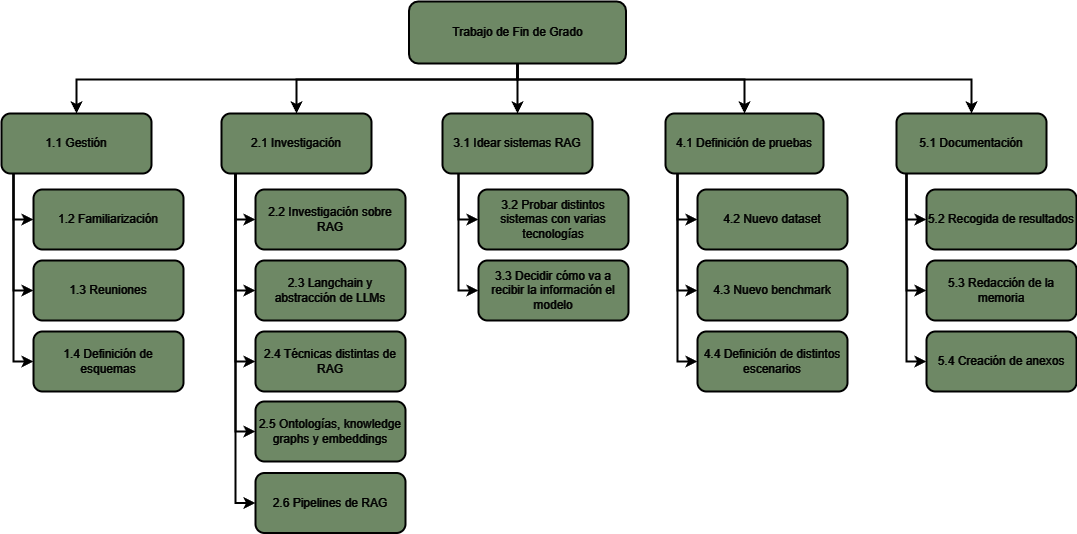
\includegraphics[width=1\textwidth]{images/tfg_edt.png}
    \caption{Esquema de división del trabajo.}
    \label{fig:edt}
\end{figure}

\subsubsection{Gestión y planificación}
En esta subsección se detallan las tareas llevadas a cabo con el fin de tener una buena gestión y planificación del proyecto.

\tabla{Reuniones.}{
    \textbf{Paquete de trabajo}: Gestión
}{
    \textbf{Tiempo estimado}: 15 horas
}{
    \textbf{Descripción}: Se realizaron reuniones semanales tanto con Mikel Egaña, como con Arkaitz Carbajo, además, con Unai López se hicieron también reuniones más extensas para revisar el estado del proyecto.
}{
    \textbf{Entregables}: Actas de reuniones
}{
   \textbf{Recursos}: Microsoft Teams en las reuniones telemáticas y OneNote para la toma de notas. 
}


\subsubsection{Investigación}
Esta sección del proyecto ha sido la que más tiempo ha tomado, ya que se dedicó mucho tiempo al principio a investigar sobre el estado del arte y las tecnologías a utilizar. Además, durante la fase de desarrollo también se han realizado investigaciones para mejorar el modelo.

\tabla{Investigación sobre el funcionamiento de los LLMs.}{
    \textbf{Paquete de trabajo}: Investigación
}{
    \textbf{Tiempo estimado}: 20 horas
}{
    \textbf{Descripción}: Se investigó sobre el funcionamiento de los LLMs, cómo se entrenan y cómo se utilizan. Además, se investigó sobre los diferentes modelos de LLMs y cuál sería el más adecuado para el proyecto.
}{
    \textbf{Entregables}: Notas sobre el funcionamiento de los LLMs
}{
    \textbf{Recursos}: OneNote para la toma de notas 
}

\tabla{Langchain y abstracción de LLMs.}{
    \textbf{Paquete de trabajo}: Investigación
}{
    \textbf{Tiempo estimado}: 20 horas
}{
    \textbf{Descripción}: Durante este paquete de trabajo de consultó un curso sobre RAG y Langchain, que se utilizó de base para implementar los sistemas de RAG que se evalúan en este trabajo.
}{
    \textbf{Entregables}: Notas sobre Langchain y abstracción de LLMs
}{
   \textbf{Recursos}: ChatGPT and LangChain: The Complete Developer's Masterclass~\cite{udemy}
}

\tabla{Técnicas de RAG.}{
    \textbf{Paquete de trabajo}: Investigación
}{
    \textbf{Tiempo estimado}: 20 horas
}{
    \textbf{Descripción}: Se investigó sobre el estado del arte de sistemas de RAG y sobre cómo son utilizados en la actualidad. Además, se investigaron técnicas de recuperación de información con distintas bases de conocimiento.
}{
    \textbf{Entregables}: Notas sobre técnicas de RAG
}{
   \textbf{Recursos}: OneNote para la toma de notas 
}

\tabla{Ontologías, knowledge graphs y embeddings.}{
    \textbf{Paquete de trabajo}: Investigación
}{
    \textbf{Tiempo estimado}: 30 horas
}{
    \textbf{Descripción}: Se investigó sobre ontologías y knowledge graphs, que se consultaron también en las reuniones con Mikel Egaña. Además, se investigaron embeddings y se hicieron pruebas para determinar qué información era útil para recuperar de una base de datos vectorial. Además, se probaron distintas bases de datos vectoriales.
}{
    \textbf{Entregables}: Notas sobre ontologías, knowledge graphs y embeddings. Decisión en base de datos vectorial.
}{
   \textbf{Recursos}: OneNote para la toma de notas. Visual Studio Code para la programación
}

\tabla{Pipelines de RAG.}{
    \textbf{Paquete de trabajo}: Investigación
}{
    \textbf{Tiempo estimado}: 20 horas
}{
    \textbf{Descripción}: Se investigó sobre creación de pipelines con RAG, recuperando información de una base de conocimiento para máyor precisión generando JQL. Se probó a introducir en el benchmark el pipeline.
}{
    \textbf{Entregables}: Notas sobre RAG. Código con distintas pruebas.
}{
   \textbf{Recursos}: OneNote para la toma de notas. Visual Studio Code para la programación
}


\subsubsection{Idear sistemas RAG}
\tabla{Probar distintos sistemas con varias tecnologías.}{
    \textbf{Paquete de trabajo}: Idear sistemas RAG
}{
    \textbf{Tiempo estimado}: 50 horas
}{
    \textbf{Descripción}: Se idearon distintos sistemas de RAG con distintas tecnologías, como ontologías, knowledge graphs y embeddings. Se probaron distintas implementaciones de estas tecnologías para ver cuál era la más adecuada para el proyecto.
}{
    \textbf{Entregables}: Código con distintas pruebas
}{
   \textbf{Recursos}: Visual Studio Code para la programación 
}

\tabla{Decidir cómo va a recibir la información el modelo.}{
    \textbf{Paquete de trabajo}: Idear sistemas RAG
}{
    \textbf{Tiempo estimado}: 20 horas
}{
    \textbf{Descripción}: Decidir, para cada implementación, cómo podría recibir la información el modelo, cómo extraerla de cada base de conocimiento y cómo presentarla.
}{
    \textbf{Entregables}: Código con distintas pruebas
}{
   \textbf{Recursos}: Visual Studio Code para la programación 
}

\subsubsection{Definición de pruebas}
Durante esta sección se definieron las pruebas que se iban a realizar para evaluar la calidad de cada una de las alternativas. Se ideó un nuevo conjunto de datos y se modificó el código del benchmark para ajustarlo al pipeline de RAG y permitir que sea replicable.

\tabla{Creación de nuevo Dataset.}{
    \textbf{Paquete de trabajo}: Definición de pruebas
}{
    \textbf{Tiempo estimado}: 2 horas
}{
    \textbf{Descripción}: Se creó un nuevo conjunto de datos con 100 preguntas, que se utilizó para evaluar las distintas alternativas propuestas. Además, se utilizó un dataset existente en Hugging Face~\cite{datasetHF} para complementar el conjunto de datos.
}{
    \textbf{Entregables}: Nuevo conjunto de datos, archivo CSV.
}{
   \textbf{Recursos}: Visual Studio Code para la programación
}

\tabla{Definición de distintos escenarios.}{
    \textbf{Paquete de trabajo}: Definición de pruebas
}{
    \textbf{Tiempo estimado}: 5 horas
}{
    \textbf{Descripción}: Se definieron distintos escenarios para evaluar las distintas alternativas propuestas. Se evaluó cómo debería ser el entorno de pruebas de Jira sobre el que se debería trabajar, con intención de aproximar el estudio a la realdiad en una empresa. Se definieron los criterios de evaluación y se crearon las pruebas para cada uno de los escenarios.
}{
    \textbf{Entregables}: Ninguno
}{
   \textbf{Recursos}: Visual Studio Code para la programación
}{}{}{}{}

\tabla{Nuevo benchmark.}{
    \textbf{Paquete de trabajo}: Definición de pruebas
}{
    \textbf{Tiempo estimado}: 5 horas
}{
    \textbf{Descripción}: Se modificó el código del benchmark para ajustarlo al pipeline de RAG y permitir que sea replicable. Se añadieron las pruebas con el nuevo conjunto de datos y se realizaron pruebas con el nuevo conjunto de datos.
}{
    \textbf{Entregables}: Código modificado del benchmark
}{
   \textbf{Recursos}: Visual Studio Code para la programación
}

\subsubsection{Documentación}
Esta sección describe cómo se realizó el proceso de documentación, tras la revisión de notas tomadas a lo largo del proyecto y la consulta con los tutores. 

\tabla{Recogida de resultados.}{
    \textbf{Paquete de trabajo}: Documentación
}{
    \textbf{Tiempo estimado}: 10 horas
}{
    \textbf{Descripción}: Se lanzan los distintos escenarios definidos y se recogen los resultados de las pruebas realizadas.
}{
    \textbf{Entregables}: Resultados de las pruebas
}{
   \textbf{Recursos}: Visual Studio Code para la programación
}
\tabla{Redacción de la memoria.}{
    \textbf{Paquete de trabajo}: Documentación
}{
    \textbf{Tiempo estimado}: 50 horas
}{
    \textbf{Descripción}: Teniendo en cuenta la toma de notas a lo largo de todo el proyecto, la valoración de distintas aproximaciones y la consulta con tutores, se redactó la memoria acorde a lo que se había planeado al principio del proyecto
}{
    \textbf{Entregables}: Memoria del trabajo de fin de grado.
}{
   \textbf{Recursos}: Visual Studio Code para la redacción de la memoria. Compilador LaTeX.
}

\tabla{Creación de anexos.}{
    \textbf{Paquete de trabajo}: Documentación
}{
    \textbf{Tiempo estimado}: 5 horas
}{
    \textbf{Descripción}: Se crearon los anexos de la memoria, que incluyen el código del benchmark y los resultados de las pruebas realizadas.
}{
    \textbf{Entregables}: Anexos de la memoria.
}{
   \textbf{Recursos}: Visual Studio Code para la redacción de la memoria. Compilador LaTeX.
}